\documentclass[paper=a4, fontsize=11pt,twoside]{article}

% -------------------------------------------------------------------- 
% General Page Layout
% --------------------------------------------------------------------
\usepackage[a4paper]{geometry} 
\usepackage[parfill]{parskip}
\setlength{\oddsidemargin}{5mm}  % Remove 'twosided' indentation
\setlength{\evensidemargin}{5mm}

% --------------------------------------------------------------------
% Encoding and Language Settings
% --------------------------------------------------------------------
\usepackage[T1]{fontenc} 
\usepackage[utf8]{inputenc}   
% encoding may need to be changed depending on the system
\usepackage[swedish]{babel} 
\usepackage{lipsum} % Lorem Ipsum
\usepackage[normalem]{ulem} %strike-out text \sout{}

% --------------------------------------------------------------------
%  Utilities (colors, links, pictures, ect...)
% --------------------------------------------------------------------
\usepackage{xcolor}
\usepackage{hyperref}
\usepackage{graphicx}
\usepackage{amssymb}
\usepackage{epstopdf}
\usepackage[round]{natbib}
\usepackage{float}
\DeclareGraphicsRule{.tif}{png}{.png}{`convert #1 `dirname #1`/`basename #1 .tif`.png}

% -----------------------------------------------------------------------------%
% Title Page / Document Class Definitions (Please Don't Play With This)
% -----------------------------------------------------------------------------%
	
% Table of contents depth = section & subsection
\setcounter{tocdepth}{2}
																								
% Horizontal rule
\newcommand{\HRule}[1]{\rule{\linewidth}{#1}}   															
																											
% Document Number
\newcommand{\documentNumber}[1]{\centering PUSP1742#1 \\[1.0cm]}	 										
																											
% Document Version
\newcommand{\documentVersion}[1]{\centering \small{v.#1} \\[1.0cm]}

% Group Responsible
\newcommand{\documentResponsible}[1]{\centering  Ansvarig Grupp: #1}

% Document Creator Group
\newcommand{\documentCreator}[1]{\centering Uppgjord Av: #1}	 									
																										
% Title
\makeatletter \def\printtitle{ {\centering \@title\par}} \makeatother
																											
% Author .. not really used, but it can stay in case
\makeatletter \def\printauthor{ {\centering \large \@author}} \makeatother
																											
\newcommand{\grouptitlepage}[4]{ 
	\title{
		\documentNumber{#1}																						
		\documentVersion{#2}																				
		\HRule{0.5pt} \\ % Upper rule 
		\LARGE \textbf{\uppercase{#3}} \\
		\large \textbf{\uppercase{ETSF20 Grupp 2}} 
		\HRule{2pt} \\ [1.5cm]    
		\normalsize            
		\documentResponsible{#4} \\ 
		\documentCreator{#4}  
	}																							
	\maketitle																							
	\thispagestyle{empty} 																					
	\newpage 
}
% \grouptitlepage{doc number}{Version Number}{doc title}{group responsible for
% doc}
% --------------------------------------------------------------------------------%
% Title Page / Document Class Definitions (Please Don't Play With This)
% --------------------------------------------------------------------------------%


% \date{}                                            
% Activate to display a given date or keep commented for current date


% -------------------------------------------------------
% DOCUMENT START (YOU CAN IGNORE EVERYTHING ABOVE HERE)
% -------------------------------------------------------
\begin{document}

% ---------------------------------------------------------------------------------------------------------------------------------------
% Title Page START: \grouptitlepage{doc number}{Version Number}{doc title}{group responsible for doc}		
% ---------------------------------------------------------------------------------------------------------------------------------------
\grouptitlepage
%Document Code Number (same as time reports)
{17}
%Document Version Number										
{1.0}
%Document Title		Dokumentmall							
{SVVR - Testrapport}
%Group Responsible For Document									
{(TG) Test Grupp} %ö
% -------------------------------------------------------------------------------------------------------------
% Title Page END				
% -------------------------------------------------------------------------------------------------------------
\tableofcontents
\section{Sammanfattning}
Sammanfattningsvis så ska det om testningen sägas att den inte helt har hållit sig till vattenfallsmetoden. Detta då UG har varit mycket aktiva och duktiga samt velat försäkra sig om att deras arbete var väl utfört. De gjorde att de redan innan TG han färdigställa och leverera testprotokollen i vissa tillfällen redan åtgärdat de fel som fanns dokumenterade. Det sista testprotokollet som TG genererade var felfritt i den mening att alla FT från SVVI som inte utgått uppfylldes detta oavsett på vilket sätt det uppnåtts.

\section{Testen}
Testen har genomförts på systemet sen dess att det fanns ett körbart projekt. Första versionen av systemet innehöll ett par fel och dessa skrevs ner i ett testprotokoll(appendix). Medan den första testningen pågick fortsatte utvecklingen av projektet vilket ledde till att flertalet av felen från det första testprotokollet hade åtgärdats innan protokollet var färdigt. Det ledde till att testprotokoll ett blev irrelevant.  Detta uppradades om än i mindre utsträckning under test två. Test två genererade testprotokoll två(appendix). Utifrån det testprotokollet genererades problemrapporter som ledde till att de felen som fanns och inte hade åtgärdats av UG medan testningen pågick, åtgärdades enligt FKG:s beslut.

Den tredje testningen genomfördes efter det att UG tvingats göra ändringar efter Anders Bruces kommentarer om en namnändring på war filen som skickades in. Det gjorde att det uppkom en del problem som troligtvis inte hade uppkommit annars då dessa problem inte fanns med i testprotokoll två. Dessa fel finns med i testprotokoll tre(appendix ). Felen i detta rapporterades till FKG och lämpliga ändringar utfördes. Innan leverans genomfördes ett sista regressionstest för att säkerställa kvaliteten på systemet. En problemrapport genererades (appendix) denna innehöll inga fel och systemet ansågs därmed leveransklart.

\section{Testprocess}
Inför testning så var det känt att FT19-FT23 i SVVI utgick. Då det inte fanns möjlighet för UG att implementera funktionaliteten som efterfrågas där. FT17 och FT18 testades inte som FT1-FT16 då de inte var funktionstester. De sågs över för att kontrollera dess korrekthet och att systemet uppfyllde även de kraven. I FT12 som refererar till tabell 8.3 i SVVS så utgick punkt (e). Detta av samma anledning som FT19-FT23 i SVVI.

De rådande omständigheterna gjorde att det inte var aktuellt med annat än regressionstest. Detta då flertalet åtgärder skedde simultant som testningen pågick vid flertalet av testtillfällena.
%\newpage
\section{Appendix: Protokoll}

\begin{figure}[h]
\centering
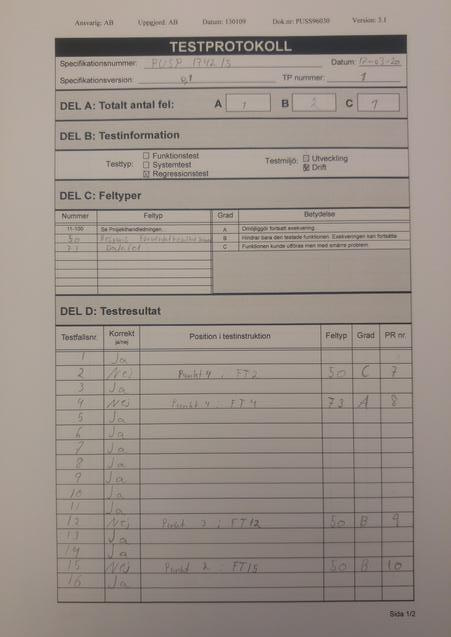
\includegraphics[width=0.65\linewidth]{test1.jpg}
\caption{Testprotokoll 1}
\label{fig:20170322135702}
\end{figure}

\begin{figure}[h]
\centering
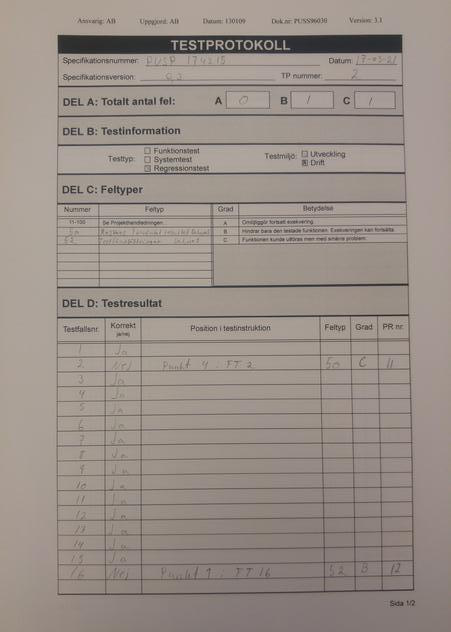
\includegraphics[width=0.65\linewidth]{test2.jpg}
\caption{Testprotokoll 2}
\label{fig:20170322135648}
\end{figure}

\begin{figure}[h]
\centering
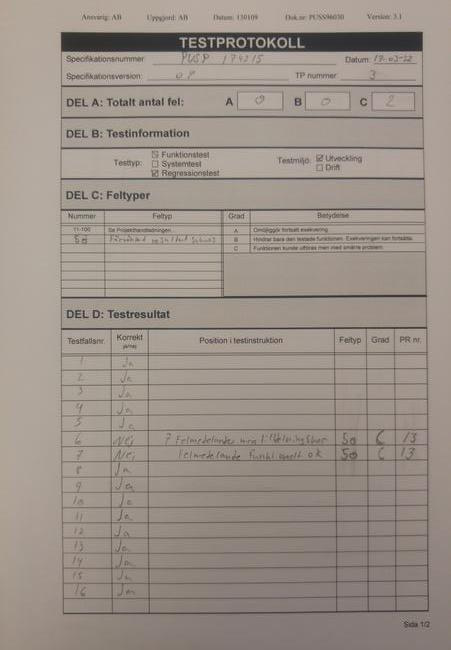
\includegraphics[width=0.65\linewidth]{test3.jpg}
\caption{Testprotokoll 3}
\label{fig:20170322135641}
\end{figure}

\begin{figure}[h]
\centering
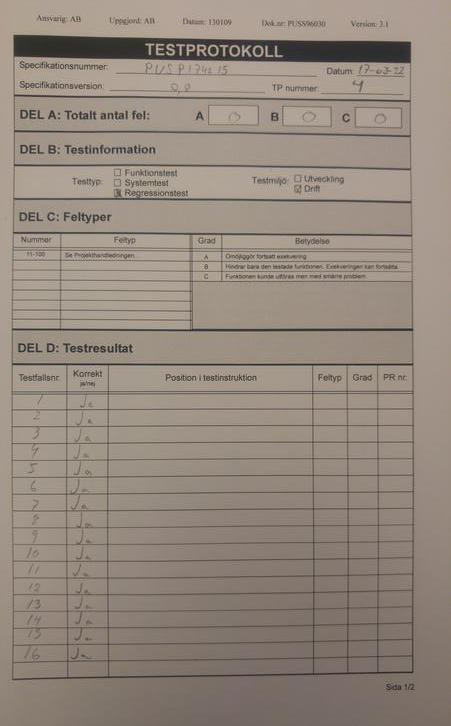
\includegraphics[width=0.65\linewidth]{test4.jpg}
\caption{Testprotokoll 4}
\label{fig:20170322135632}
\end{figure}

\begin{figure}[h]
\centering
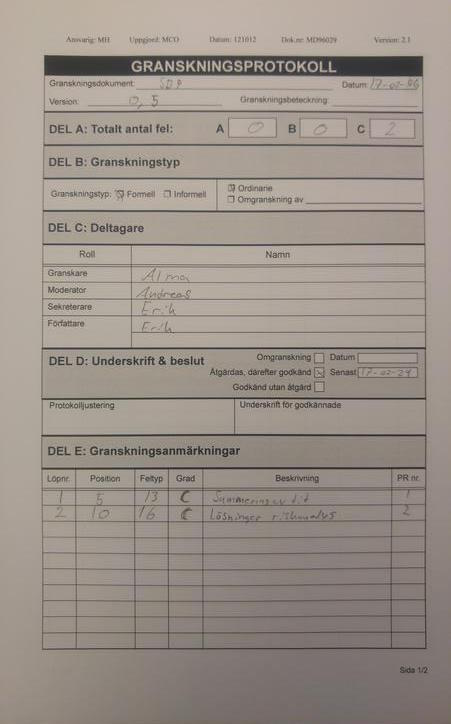
\includegraphics[width=0.65\linewidth]{SDP.jpg}
\caption{Granskningsprotokoll SDP}
\label{fig:20170322135626}
\end{figure}

\begin{figure}[h]
\centering
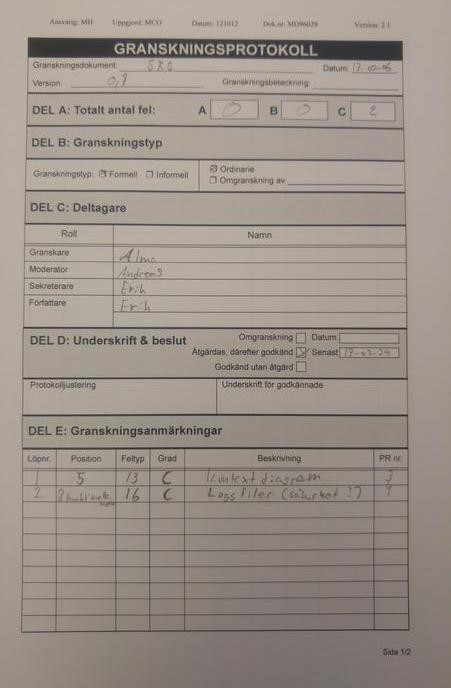
\includegraphics[width=0.65\linewidth]{SRS.jpg}
\caption{Granskningsprotokoll SRS}
\label{fig:20170322135735}
\end{figure}

\begin{figure}[h]
\centering
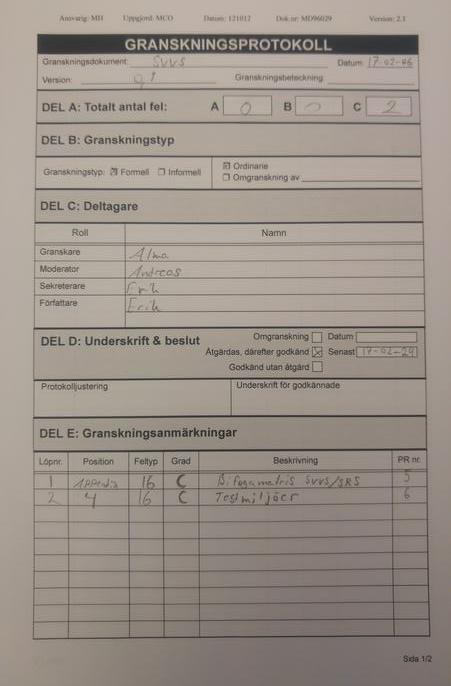
\includegraphics[width=0.65\linewidth]{SVVS.jpg}
\caption{Granskningsprotokoll SVVS}
\label{fig:20170322135723}
\end{figure}

\begin{figure}[h]
\centering
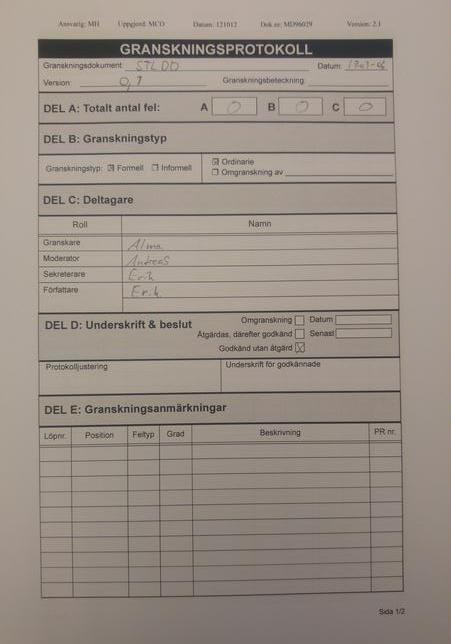
\includegraphics[width=0.65\linewidth]{STLDD.jpg}
\caption{Granskningsprotokoll STLDD}
\label{fig:20170322135715}
\end{figure}

\begin{figure}[h]
\centering
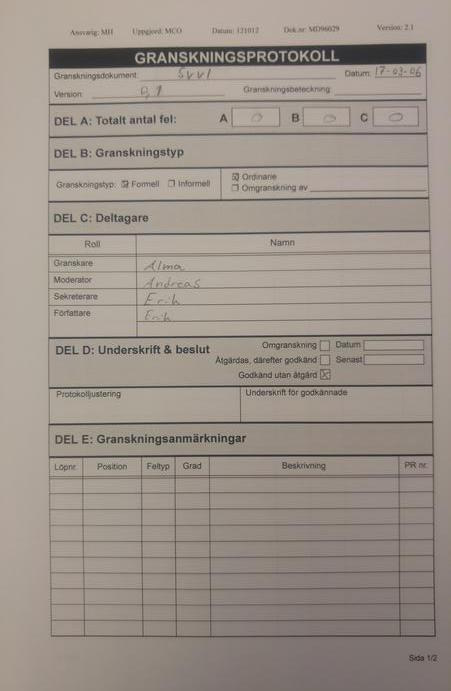
\includegraphics[width=0.65\linewidth]{SVVI.jpg}
\caption{Granskningsprotokoll SVVI}
\label{fig:20170322135709}
\end{figure}

\end{document}